% Use the document class appropriate to your language and leave the other
% line commented out
%\documentclass{acm_proc_article-sp-german}
\documentclass{acm_proc_article-sp}

% These two lines help to keep enumerations and itemizations compact.
% Try commenting them out if you want to see the effect.
\usepackage{enumitem}
\setlist{nolistsep}

% The next two commands are for the code display example. Look into the
% documentation of the listings package for other configurations, in
% particular for a list of supported programming languages.
\usepackage{listings}
\lstset{language = C, 
        numbers=left, 
        numberstyle=\tiny,
        columns=fullflexible, 
        basicstyle=\sf, 
        xleftmargin = 0.5 cm}

% Display subfigures
\usepackage{subfig}

% Generate PDF hyperlinks when referencing sections and stuff. Also, get
% rid of the need to 
\usepackage{hyperref}

% This is the name of the folder you are placing your graphics files in.
% Defining it here makes LaTeX look for files there without you having
% to specify the folder again throughout the document.
\graphicspath{ {./graphics/} }

\begin{document}

\title{A Mini LaTeX Primer}
\numberofauthors{1}
\author{
	\alignauthor
	Horst-Günther Gugelhupf\\
	\affaddr{Department of Computer Science}\\
	\affaddr{Christian-Albrechts-Universit\"at zu Kiel}\\
	\affaddr{googlehupf@informatik.uni-kiel.de}
}

\date{\today}

\maketitle

%%%%%%%%%%%%%%%%%%%%%%%%%%%%%%%%%%%%%%%%%%%%%%%%%%%%%%%%%%%%%%%%%%%%%%%%%%
\begin{abstract}
  This file shows some basic latex features
  you might need for the seminar. 
\end{abstract}


%%%%%%%%%%%%%%%%%%%%%%%%%%%%%%%%%%%%%%%%%%%%%%%%%%%%%%%%%%%%%%%%%%%%%%%%%%
\section{Introduction}
\label{sec:introduction}

This is a section.
You can add a label
to a lot of document elements
to reference them later in the text.
In the code of this document,
we distribute each sentence
over several lines.
This is because having very long lines
make it difficult to find the differences
between two revisions of your document
when you use a version control system
such as Git.

If you want to start a new paragraph,
do it by inserting a blank line.
Never ever try to start new paragraphs
by inserting a simple\\line break.


%%%%%%%%%%%%%%%%%%%%%%%%%%%%%%%%%%%%%%%%%%%%%%%%%%%%%%%%%%%%%%%%%%%%%%%%%%
\section{Example section}
\label{sec:exampleSection}

And this is another section,
just like \autoref{sec:introduction}.
This one even has subsections,
see for example \autoref{subsec:subsectionExample}.


%%%%%%%%%%%%%%%%%%%%%%%%%%%%%%%%%%%%%%%%%%%%%%%%%%%%%%
\subsection{A subsection example}
\label{subsec:subsectionExample}

Now this is an example of a subsection.


%%%%%%%%%%%%%%%%%%%%%%%%%%%%%%%%%%%%%%%%%%%%%%%%%%%%%%
\subsection{Another subsection example}
\label{subsec:compoundSubsection}

And this is an example of another subsection.
All hail to this subsection!
However,
you should try to get by
with sections and subsections.
If you start reaching for subsubsections,
reconsider your document structure.


%%%%%%%%%%%%%%%%%%%%%%%%%%%%%%%%%%%%%%%%%%%%%%%%%%%%%%%%%%%%%%%%%%%%%%%%%%
\section{Some helpful features}

You might want to itemize things.
For example,
this is a good burger:
\begin{itemize}
  \item a fresh bun,
  \item sappy, grilled minced meat,
  \item cheese,
  \item onions, and
  \item barbecue sauce.
\end{itemize}

Or even enumerate them.
There are only four things
I want my burger to consist of:
\begin{enumerate}
  \item a fresh bun,
  \item sappy, grilled minced meat,
  \item cheese,
  \item onions, and
  \item barbecue sauce.
\end{enumerate}

Or you might even need a description:
\begin{description}
  \item [bun] The bun has to be fresh and crispy.
  \item [meat] The minced meat should be grilled on real fire.
  \item [cheese] A quarter pounder with cheese is best with cheese in it.
  \item [onions] They are the only vegetables I need on a burger.
  \item [barbecue sauce] Is better than mayonnaise.
\end{description}

There are two lines in the header of this file
that help to keep things compact around here.
If you do not mind spending more vertical space,
you can comment them out.
In general,
only use lists if necessary.
If you simply want to enumerate a bunch of
words, terms, expressions, or phrases,
just include them directly into your text.


%%%%%%%%%%%%%%%%%%%%%%%%%%%%%%%%%%%%%%%%%%%%%%%%%%%%%%%%%%%%%%%%%%%%%%%%%%
\section{Graphics}

If you want to illustrate your text with some graphics
(which is a good idea),
please add a subfolder to your repository folder,
give it a name like \texttt{images} or \texttt{graphics}
and store your pictures there
in pdf- and original Format.
Prefer vector-graphics over bitmaps
since they scale and look better
in the final paper.
To find an example of how to include your pictures,
take a look at this document's source.

\begin{figure}
  \centering
  % You don't need to include the .pdf file name extension
  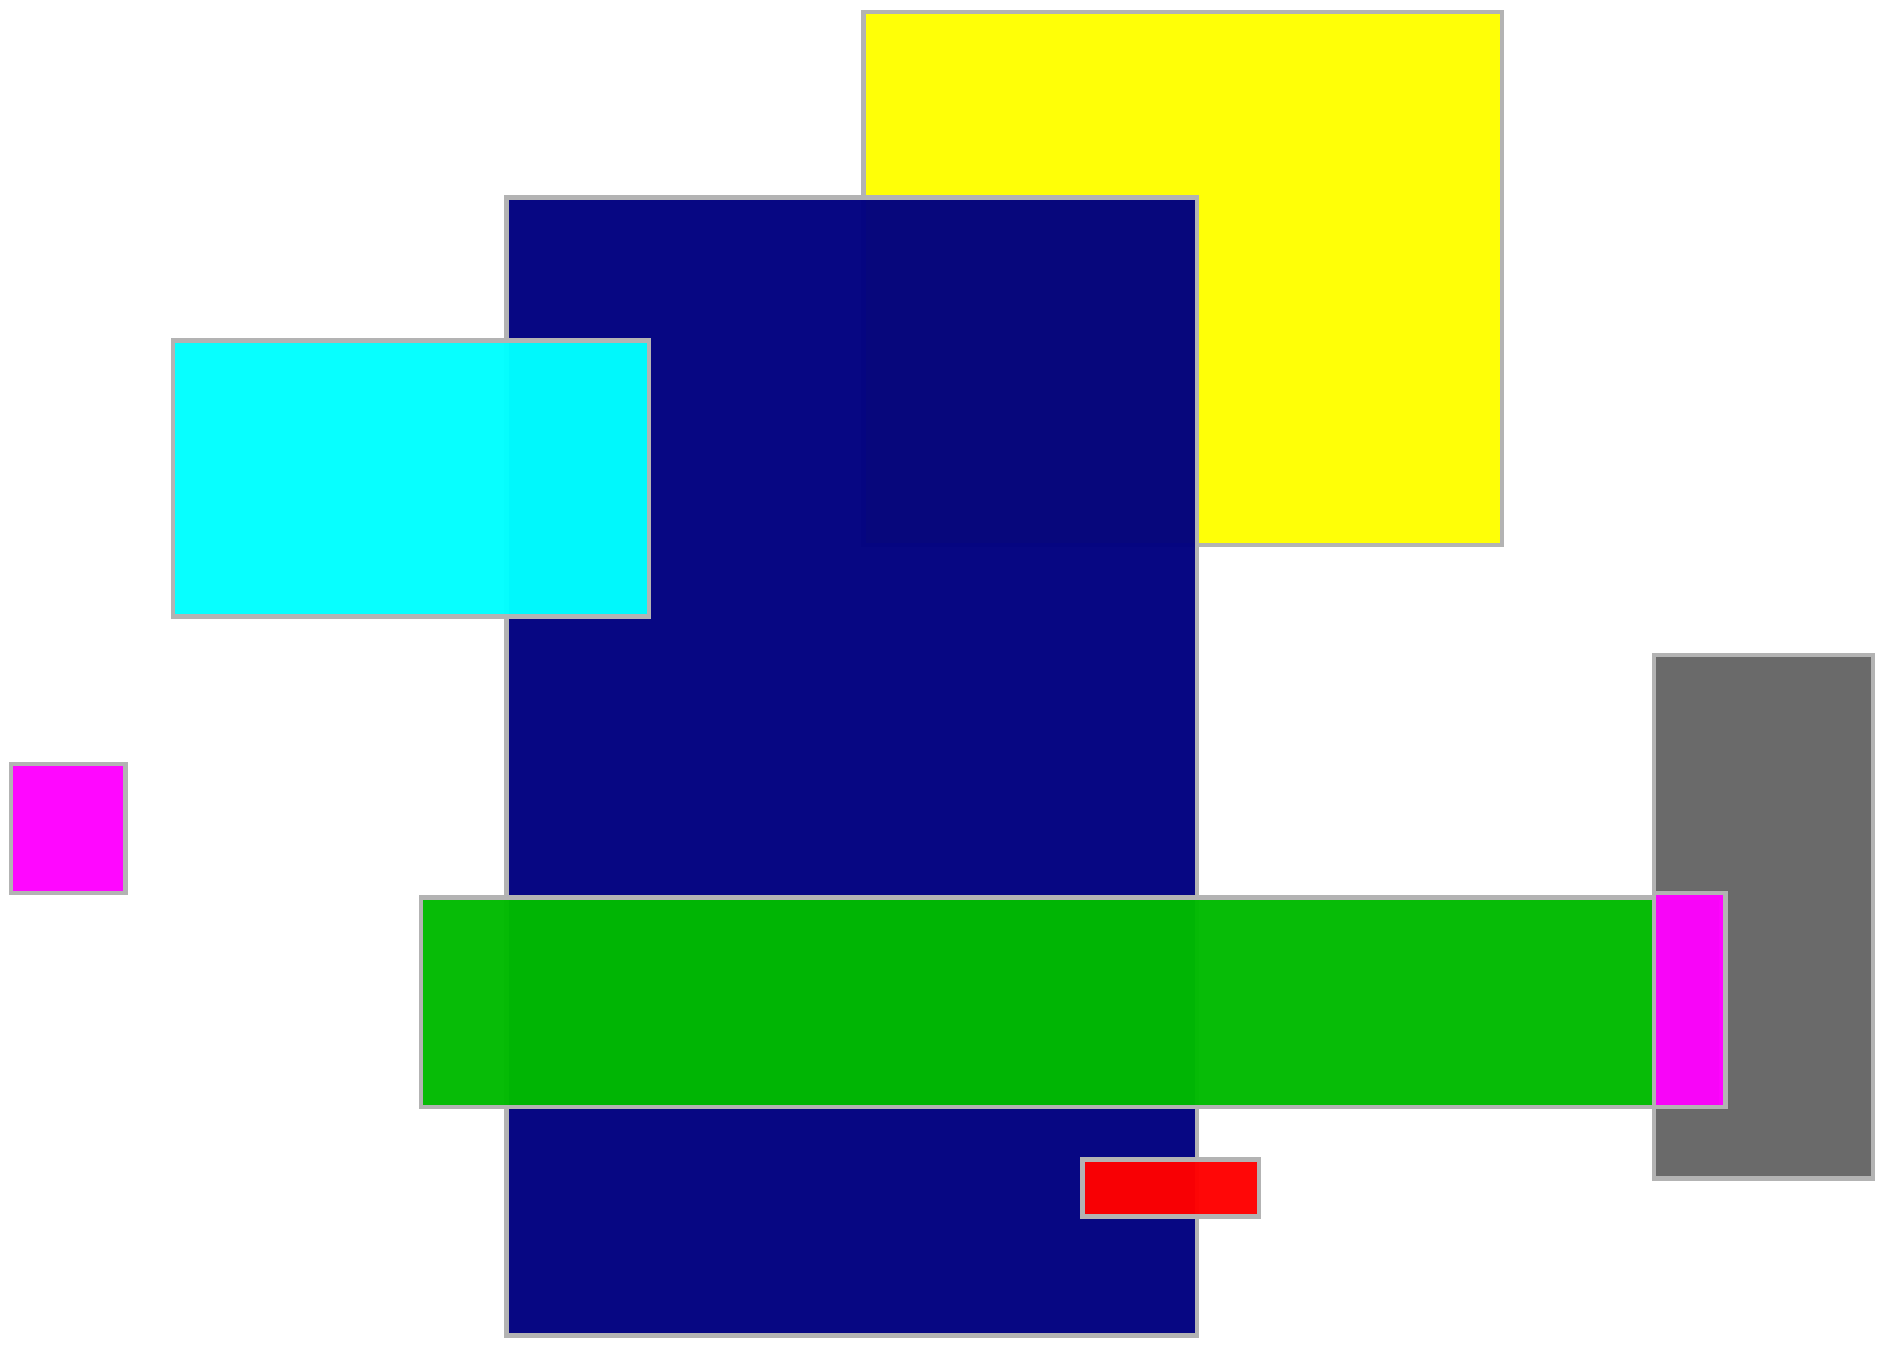
\includegraphics[scale=0.2]{drawing}
  \caption{This is an example figure.}
  \label{fig:drawing}
\end{figure}

The caption is the text
that will appear under your picture.
By changing the scale
you can adjust the size of your picture---%
if you have any labels or text in your picture,
the smallest font be nearly the same size as the caption font size.
Of course,
you will want to reference your picture in the text.
See, for example, \autoref{fig:drawing}.

If you have some pictures
that you want to discuss in combination,
you might use subfigure
as we do in \autoref{fig:twoPics}.
You can also reference each subfigure separately
in your text.

\begin{figure}
  \subfloat[]{
    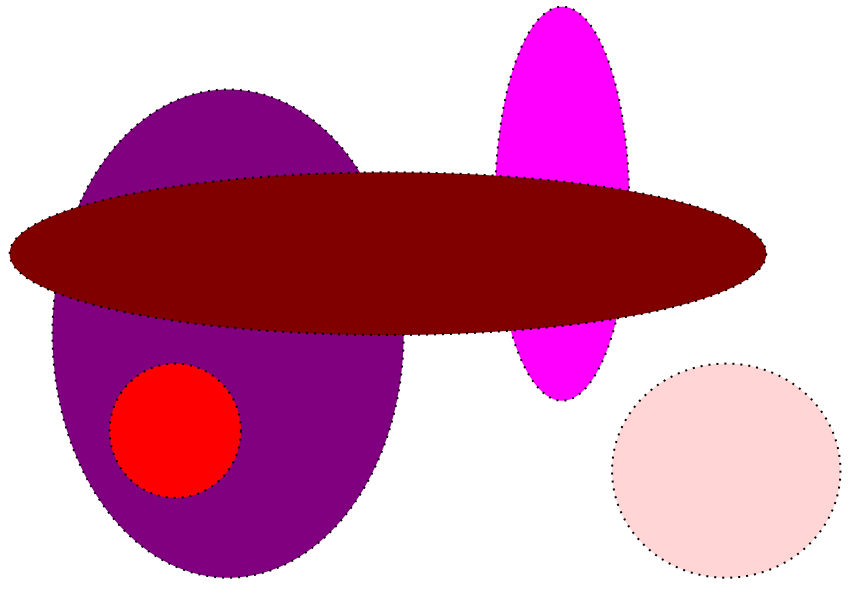
\includegraphics[scale=0.14]{ellipses}
    \label{fig:twoPics_ellipses}
  }
  \hfill
  \subfloat[]{
    
\includegraphics[scale=0.14]{abstract}
    \label{fig:twoPics_rightColors}
  }
  \caption{This is a figure
    with two subfloats in it,
    \protect\subref{fig:twoPics_ellipses}
    and \protect\subref{fig:twoPics_rightColors}.}
  \label{fig:twoPics}
 \end{figure}


%%%%%%%%%%%%%%%%%%%%%%%%%%%%%%%%%%%%%%%%%%%%%%%%%%%%%%%%%%%%%%%%%%%%%%%%%%
\section{Referring to the work of others}

If you want to cite a paper,
edit your bibliography database file \texttt{myrefs.bib}
and insert the bibtex information
of the paper you want to cite.
You can then refer to the paper like this:
As Lee has stated,
threads can be problematic~\cite{L06}.


%%%%%%%%%%%%%%%%%%%%%%%%%%%%%%%%%%%%%%%%%%%%%%%%%%%%%%%%%%%%%%%%%%%%%%%%%%
\section{Including code samples}

Here is a very basic C code example.
To customize how the code appears in the final document,
see the start of the source file of this document.

\begin{lstlisting}
#include <stdio.h>

  int main(void)
  {
    printf("Hello, World\n");
    return 0;
  }
\end{lstlisting}


%%%%%%%%%%%%%%%%%%%%%%%%%%%%%%%%%%%%%%%%%%%%%%%%%%%%%%%%%%%%%%%%%%%%%%%%%%
\section{Typesetting Equations}

You can include formulas and equations,
such as \(M = \{x \in \mathbb{N} ~|~ x < 10\}\),
in your running text.
If you want the formula
to be on its own line,
that's possible as well:
\begin{equation*}
  \sum_{i=0}^{k}\frac{y}{x_{i}}.
\end{equation*}
If you want to label equations
to refer to them in the text,
use the \texttt{equation} environment
and define a label for the equation:
\begin{equation}
  \sum_{i=0}^{k}\frac{y}{x_{i}}.
  \label{eq:le_equation}
\end{equation}
See \autoref{eq:le_equation}
for an example.
There are a lot of LaTeX equation editors on the web
which can help you write your equations.


%%%%%%%%%%%%%%%%%%%%%%%%%%%%%%%%%%%%%%%%%%%%%%%%%%%%%%%%%%%%%%%%%%%%%%%%%%
\section{Going further}

LaTeX is a powerful typesetting system that,
while perhaps a bit cumbersome to use for small documents,
will usually produce better results
than the popular office packages.
It thus pays to learn how to use it---%
even more so since chances are
you will typeset your Bachelor's or Master's thesis
using LaTeX.

The web is full of documentation.
A good starting point
is the Wikibook on LaTeX.\footnote{\url{http://en.wikibooks.org/wiki/LaTeX}}


%%%%%%%%%%%%%%%%%%%%%%%%%%%%%%%%%%%%%%%%%%%%%%%%%%%%%%%%%%%%%%%%%%%%%%%%%%
% Bibliography

% The bibliography entries are stored in "myrefs.bib"
\bibliographystyle{abbrv}
\bibliography{myrefs}

\end{document}

